\section{\textsf{PTAS} under Resource Augmentation}
\label{sec:ptas-ra}
In this section, we present a \textsf{PTAS} when the input items are fat convex objects, and we are allowed to increase the size of the given knapsack by a factor of $1+\eps$ in each dimension. Chagas et al.~\cite{MiyazawaWAOA} presented a \textsf{PTAS} for circles with resource augmentation in one dimension. Their result is based on a combination of multiple integer programs with variables for different configurations for packing parts of the given knapsack.
Our result is arguably simpler and purely based on dynamic programming.


Let $P_i$ be a two-dimensional convex object and let $r_{i}^{\mathrm{out}}(P_i)$ and $r_{i}^{\mathrm{in}}(P_i)$ be
the radius of the smallest circle containing $P_{i}$ and the radius
of the largest circle contained in $P_i$, respectively. 
We will drop $P_i$ when it is clear from the context. 
We say that $P_i$ is $f$\emph{-fat} if  $r_{i}^{\mathrm{out}}/r_{i}^{\mathrm{in}}\le f$
for some value $f \ge 1$. In the remainder of this section, we prove the following theorem.

\begin{theorem}
	\label{thm:fat-ra}
	Let \ari{$f\ge 1$}, $\eps>0$, and $d\in \N$ be constants. Given a set of $d$-dimensional $f$-fat convex input objects, there exists a polynomial time algorithm that can pack a subset of them with a total profit of \ag{$w(\OPT)$} into a knapsack $K':=[0, 1+\eps]^d$, where \ag{$w(\OPT)$} is the optimal profit that can be packed into a knapsack $K:=[0, 1]^d$.
\end{theorem}
\arir{OPT is value or set}

% Now we prove \Cref{thm:fat-ra}.
For simplicity, we first describe our algorithm in the setting where $d=2$.
Given a packing of a set of $f$-fat objects $\mathcal{P}=\{P_1, P_2, \dots, P_n\}$ in our knapsack $K=[0, 1] \times [0, 1]$, we want to show that there is also a structured packing of these objects \ari{into an augmented knapsack $K'=[0, 1+\eps]\times [0, 1+\eps]$}, defined via a discrete grid. Let $\dc>0$ be a constant to be defined later such that $1/\dc \in \mathbb{N}$. We place a two-dimensional grid inside \ari{$K'$} such that each grid cell has an edge length of $\dc$. Let $\mathcal{G}$ denote the set of all resulting grid cells. We assume first that each object $P_i \in \mathcal{P}$ is \emph{$\dl$-large}, meaning that $r^{in}(P_i) \ge \dl$ for some given constant $\dl>0$. We say that our given packing for $\mathcal{P}$ is {\em discretized} if there is a partition of $\mathcal{G}$ into sets $\{\mathcal{G}_{P_1}, \mathcal{G}_{P_2}, \dots, \mathcal{G}_{P_n}\}$ such that for each $P_i \in \P$, we have that $P_i$ is contained in the union of the cells in $\mathcal{G}_{P_i}$. Therefore, each object $P_i \in \P$ has its ``own'' set of grid cells $\mathcal{G}_{P_i}$ that contain $P_i$ and that do not intersect with any other object $P_j \in \P \setminus \{P_i\}$. 
% \textcolor{red}
{This is similar to the approach used by Miyazawa et al. \cite{MiyazawaPSSW16} for the circle bin packing problem which is also based on a hierarchical decomposition.}


\ari{We show that for an appropriate choice of $\dc$, there is a discretized packing for $\mathcal{P}$ in $K'$, i.e., if we can increase the size of our knapsack $K$ by a factor of $1+\eps$ in each dimension.}

\begin{lemma}%[$\star$]
	\label{lem:fatdisc}
	For each $f \ge 1$, $\eps>0$, and $\dl>0$, there is a value $\dc>0$ such that for any set of $\dl$-large $f$-fat convex objects $\mathcal{P}$
	that can be placed non-overlappingly inside a knapsack $K=[0, 1] \times [0, 1]$, there is a discretized packing
	for $\mathcal{P}$ inside knapsack $\ag{K'= } [0, 1+\eps] \times [0, 1+\eps]$
	based on a grid in which each edge of each grid cell has a length of $\dc$.
\end{lemma}

\begin{proof}
	\begin{figure}%[H]
		\centering 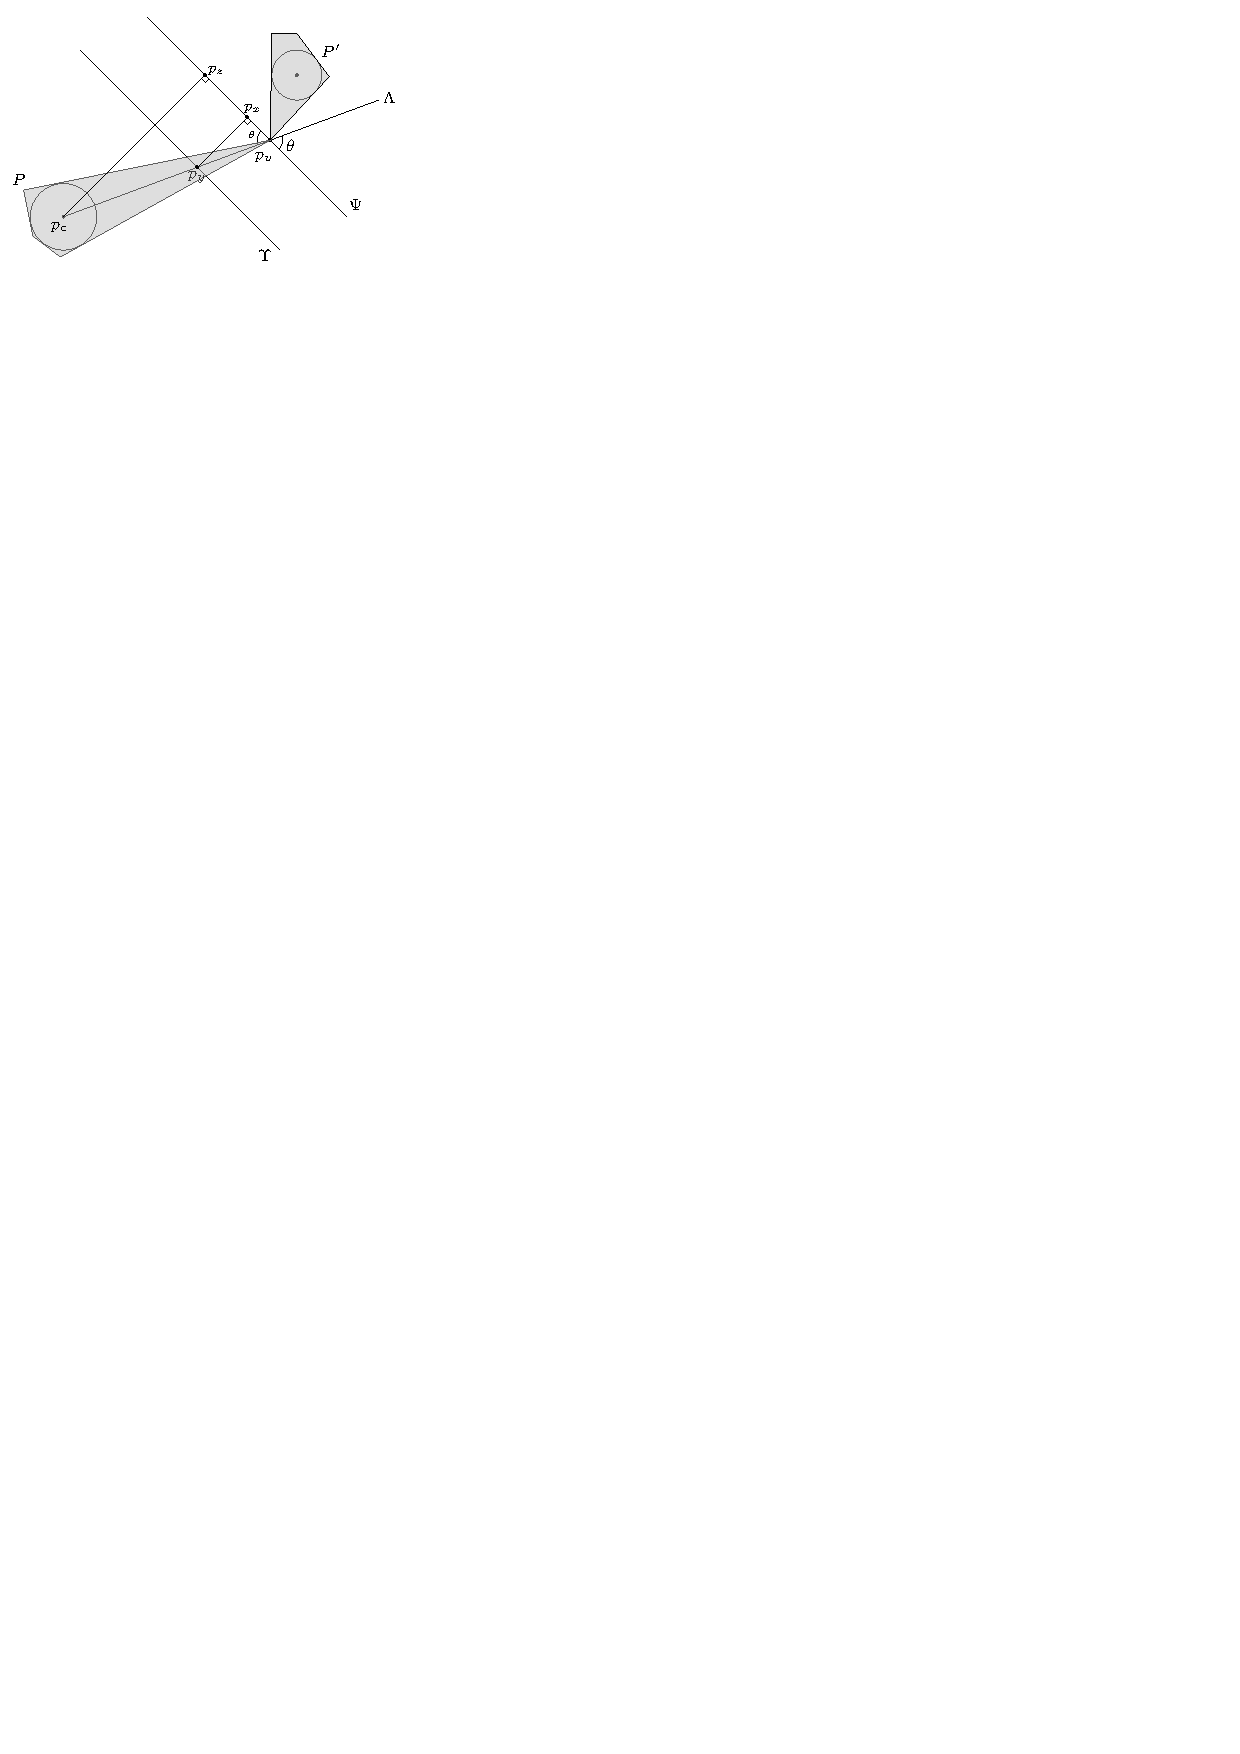
\includegraphics[width=0.6\textwidth]{Figures/aar_figure2.pdf}
		\caption{\ag{Line $\Psi$ separates the two $f$-fat and convex objects $P$ and $P'$. We construct line $\Upsilon$ such that it intersects no common grid cells with line $\Psi$. We proceed to shrink the two objects $P, P'$ by a factor of $1+\eps$ such that they cannot intersect the space between lines $\Upsilon$ and $\Psi$.}}
		\label{fig:hyperplane}
	\end{figure}

	\begin{figure}%[H]
		\centering 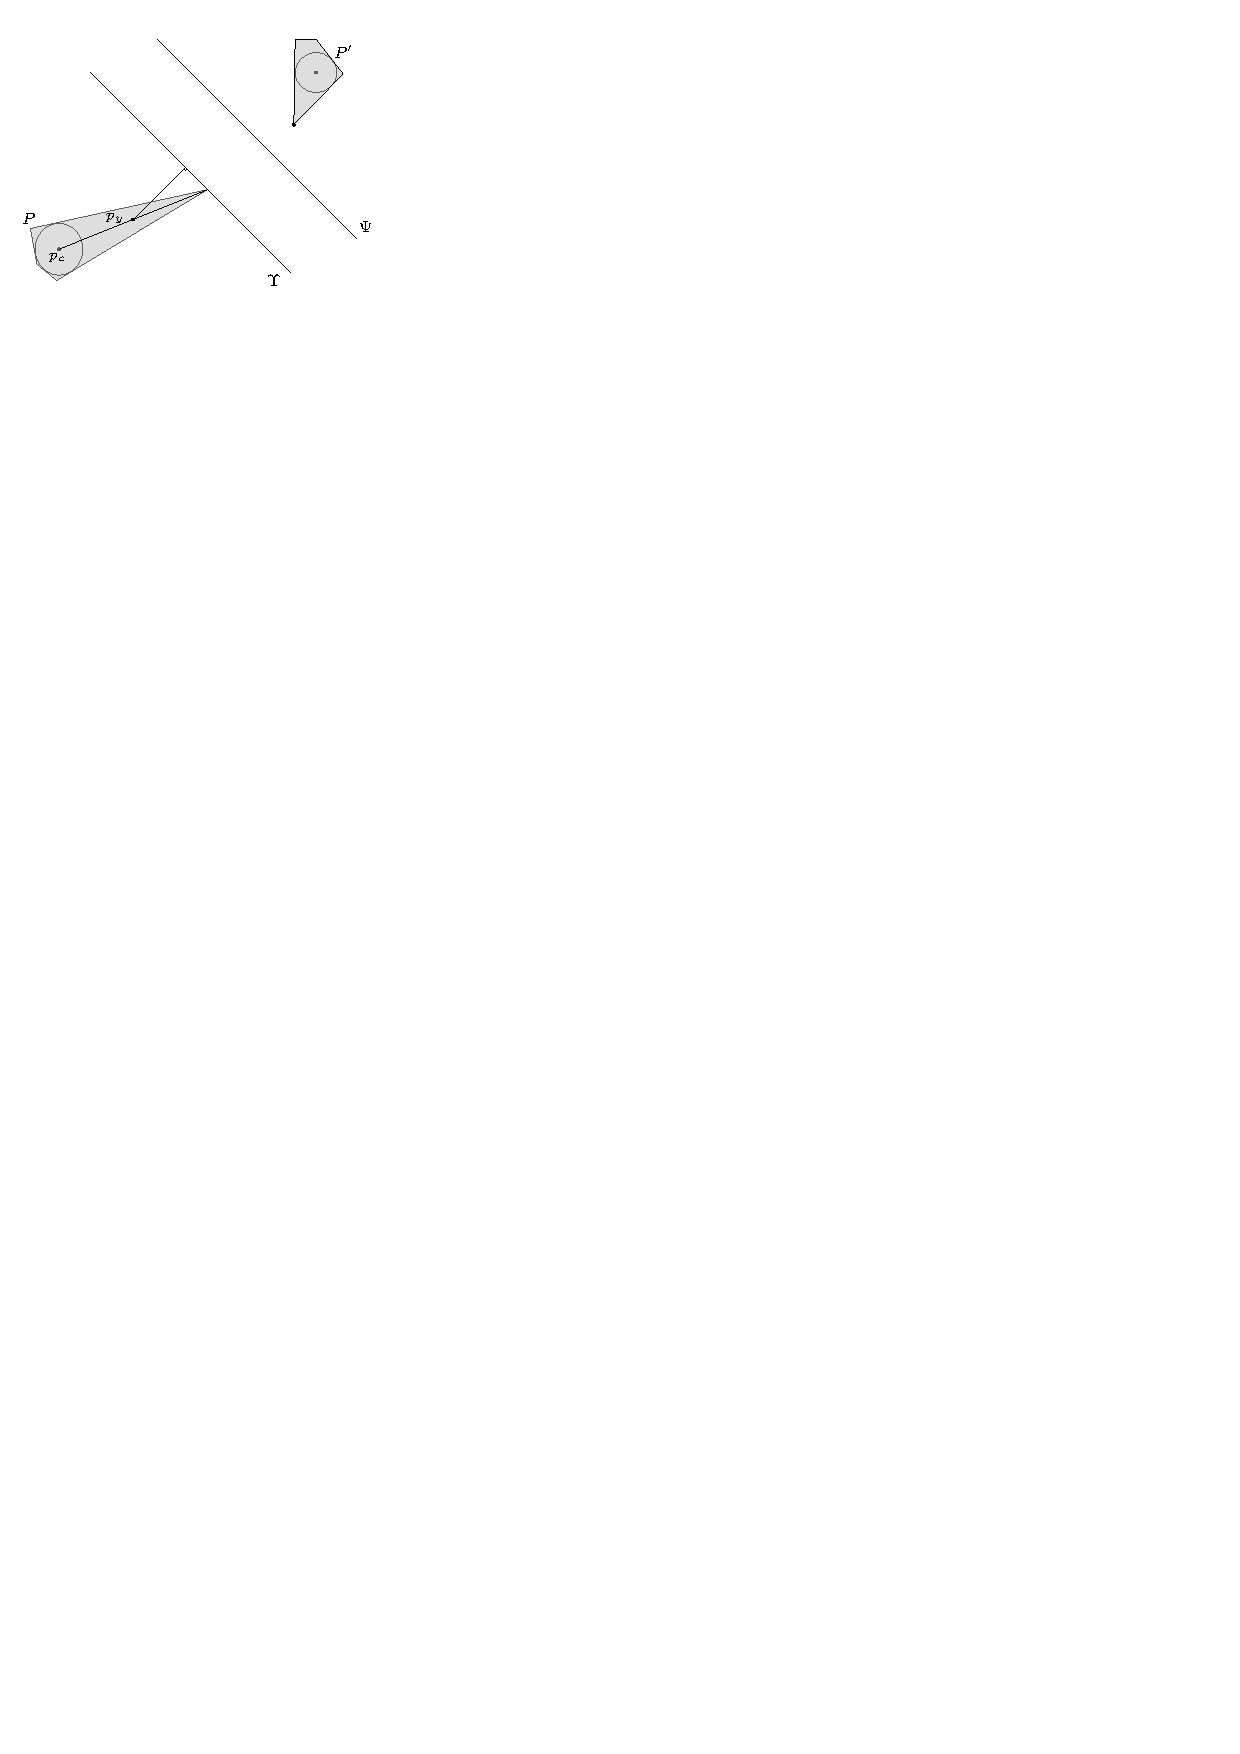
\includegraphics[width=0.6\textwidth]{Figures/aar_figure3.pdf}
		% 	\centering \includegraphics[width=0.3\textwidth]{Images/Final/corner}
		% Scale image to the width of the text
		\caption{\ag{$P,P'$ are shrunk so that they cannot intersect the space between the lines $\Upsilon$ and $\Psi$.}}
		\label{fig:zoomed}
	\end{figure}
	
	Let $P, P' \in \mathcal{P}$ be two $f$-fat convex $\dl$-large objects packed inside the knapsack.
	Then by {\em separating hyperplane theorem for convex objects}~\cite{boyd2004convex}, we know that there is a line $\Psi$ containing a point $p_v$ on \agtwo{the} boundary of $P$, and $\Psi$ separates $P$ from $P'$  (see Figure \ref{fig:hyperplane}). 
	Now, intuitively, increasing the size
	of the knapsack by a factor of $1+\eps$ is equivalent to shrinking
	the objects in $\mathcal{P}$ by a factor of $1+\eps$. So, we want to find the right constraints such that after shrinking $P$ and $P'$ do not share any grid cell. 
	Let the center of the incircle (of radius $r^{in}$) contained in $P$ be $p_c$ and the line joining $p_c$ and $p_v$ be $\Lambda$. 
	Let the foot of the image of the point $p_c$ on line $\Psi$ be the point $p_z$.  Now the length of line segment $\overline{p_c p_z}  := |\overline{p_c p_z}| \geq r^{in}$ and $|\overline{p_c p_v}| \leq 2 f r^{in}$, as the diameter of $P$ is at most $2 f r^{in}$. Hence, the angle $\theta$ between $\Psi$ and $\Lambda$ is at least ${\sin}^{-1}(\frac{1}{2f})$. Consider points $p_x$ on $\Psi$ and $p_y$ on $\Lambda$ such that $|\overline{p_x p_y}| = \sqrt2 \dc$ and the line  joining $p_x, p_y$ is parallel to the line joining $p_c p_z$. Let $\Upsilon$ be the line passing through $p_y$ and parallel to $\Psi$.  
	Then any point on $\Psi$ does not share a grid cell with any point on $\Upsilon$. 
	Also, $|\overline{p_y p_v}| =  \frac{|\overline{p_c p_v}|}{|\overline{p_c p_z}| } \cdot  {|\overline{p_x p_y}| } \le \frac{2 f r^{in}}{r^{in}} \sqrt2 \dc \le 2 \sqrt2 f \dc$.
	Now we want to shrink  $P$ by $(1+\eps)$ factor keeping $p_c$ at the same position such that the shrunk version of $P$ lies completely within one side of $\Upsilon$ \ag{(see Figure \ref{fig:zoomed})}.
	After shrinking, $\overline{p_c p_v}$ gets smaller by $\eps |\overline{p_c p_v}| \ge \eps r^{in} \ge \eps \dl$.
	Now we choose $\dc$ such that $\dc \le \frac{\eps}{2 \sqrt2 f} \cdot \dl$.
	Thus we satisfy $\eps |\overline{p_c p_v}| \ge \eps \dl \ge  2 \sqrt2 f \dc  \ge  |\overline{p_y p_v}|$ and this ensures that the shrunk down version of $P$ and $P'$ do not share any grid cell.  
	We assign each polygon to the grid cells that it intersects with. 
	Hence this process leads to a discretization such that the no grid cell is intersected by two polygons.
\end{proof}

\begin{figure}
	\begin{center}
		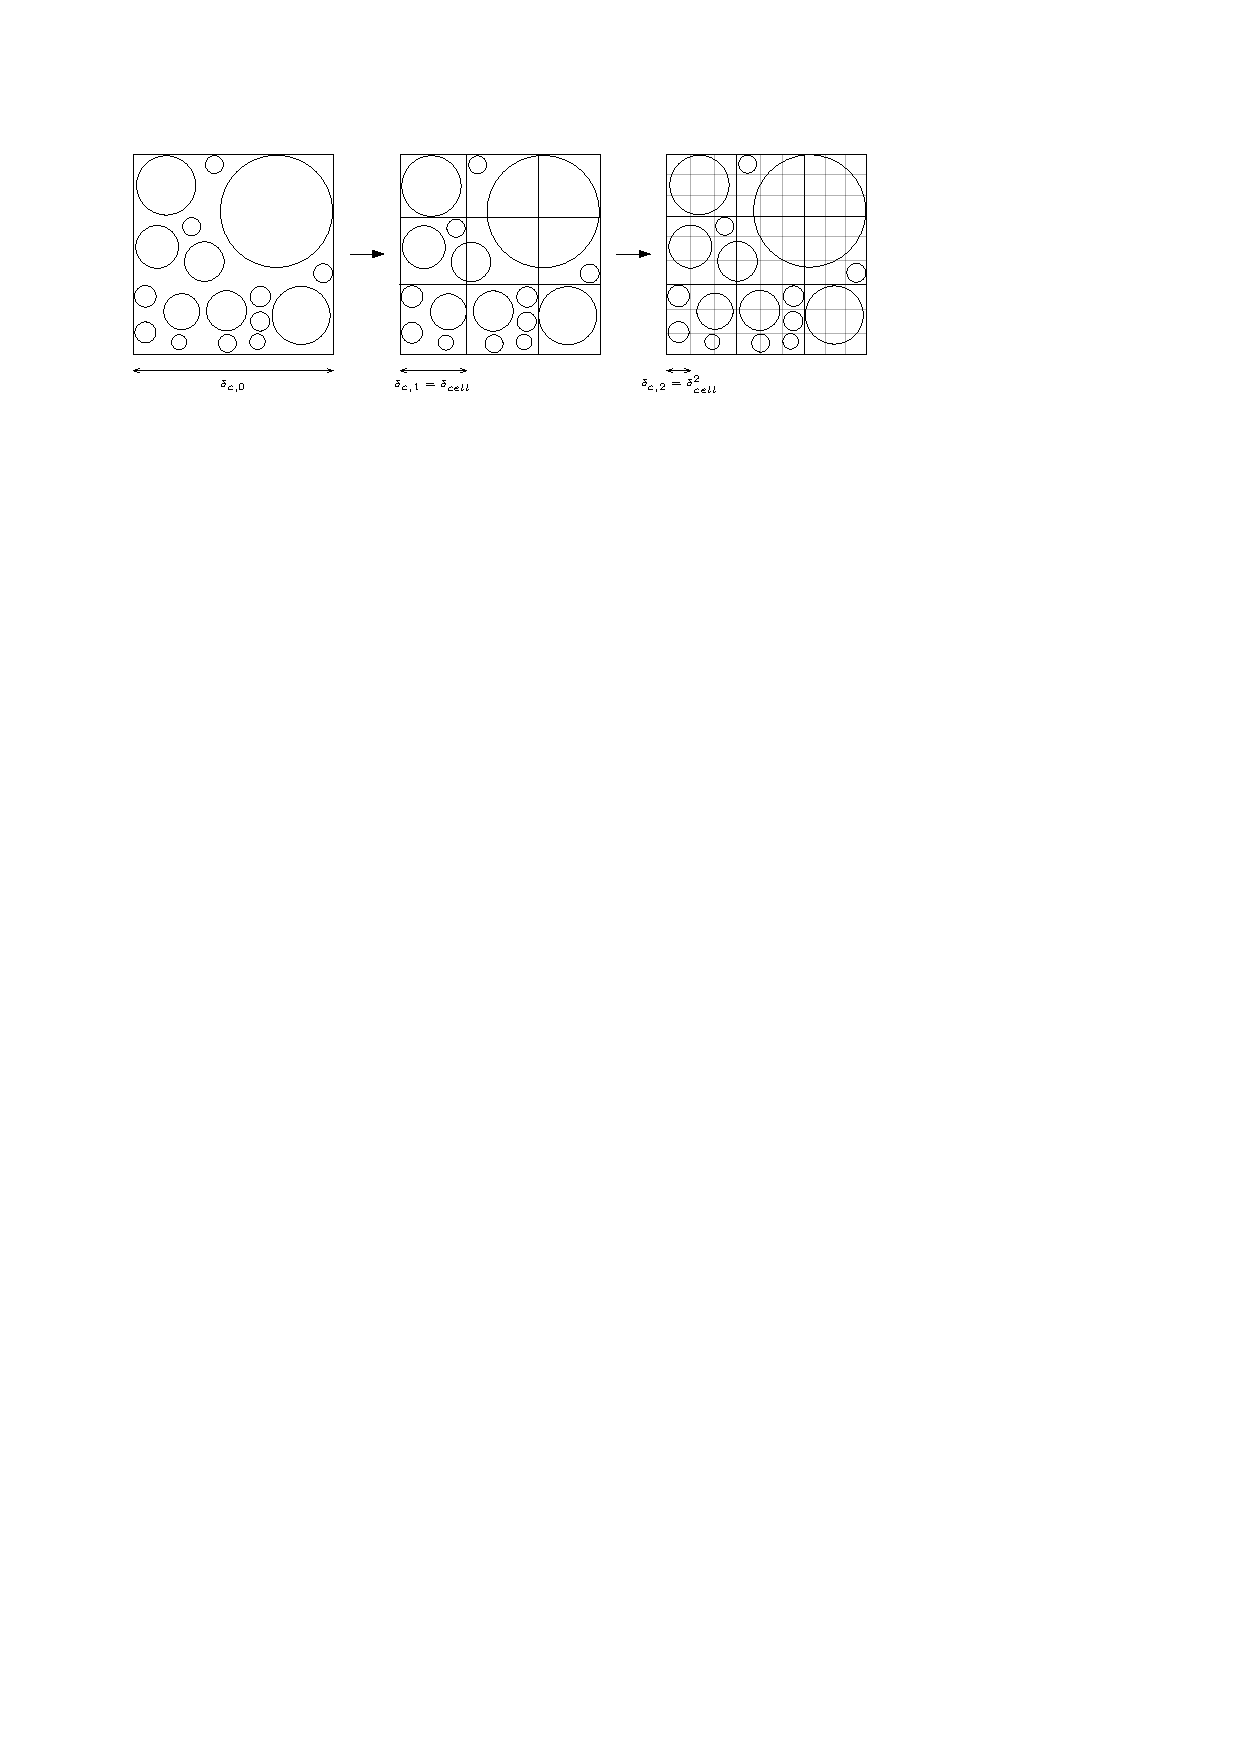
\includegraphics[width=14cm]{Figures/discretized_packing_example.pdf}
		\caption{An illustration of a hierarchical grid. The second level gridcells in the example define a `discretized' packing of the circles, i.e., no two circles share a common gridcell.}
		\label{fig:discretized_packing_example}
	\end{center}
\end{figure}

Next, we argue that there is also a structured packing for fat objects
that are not necessarily all (relatively) large. Let $\dl,\dc,\ds>0$
be constants to be defined later (they will depend on $\eps$
which will denote the amount by which we increase the size
of our knapsack). We place now a \emph{hierarchical} two-dimensional grid
with multiple levels. We define that
the whole knapsack $K$ is one grid cell of level 0 of side length
$\delta_{c,0}:=1$. For each level $\ell\ge1$, we define grid cells
whose edges all have a length of $\delta_{c,\ell}:=\dc\delta_{c,{(\ell-1)}}$.
%\dc\delta_{c,{(\ell-1)}}^{6}$.
Recursively, for each $\ell\ge1$ %we define $\delta_{c,\ell}:=\dc\delta_{c,{(\ell-1)}}^{6}$
we partition each grid cell of level $\ell-1$ into ${1/\dc^{2}}$
grid cells of level $\ell$ with side length $\delta_{c,\ell}$ each. See Figure  \ref{fig:discretized_packing_example}.
Similarly as before, we want that there is a partition of the grid
cells such that for each object $P\in\P$ there is a set of grid cells
$\G_{P}$ that contain $P$ and that are disjoint from the grid cells
$\G_{P'}$ for each object $P'\in\P\setminus\{P\}$. Also, we want
that all grid cells in $\G_{P}$ are of the same level, that their
size is comparable to the size of $P$, and that the number of grid
cells in $\G_{P}$ is bounded. To ensure this, we group the objects
$P\in\P$ according to their respective values $r^{\ag{in}}(P)$ which
we use as a proxy for their sizes. Formally, we define $\delta_{small,0}:=1$
and for each level $\ell\ge1$ we define $\delta_{large,\ell}:=\dl{\delta_{c,{(\ell-1)}}}$
and $\delta_{small,\ell}:=\ds\delta_{c,{(\ell-1)}}$. %


For each level $\ell$ we define
\begin{itemize}
 \item $L_{\ell}$ to be all objects
$P\in\P$ with $r^{\ag{in}}(P)\in(\delta_{large,\ell},\delta_{small,{(\ell-1)}}]$;
intuitively, they are ``large'' for level $\ell$,
\item $M_{\ell}$ to be all objects $P\in\P$ with $r^{in}(P)\in(\delta_{small,\ell},\delta_{large,\ell}]$.
\end{itemize}

\begin{figure}
    \centering
    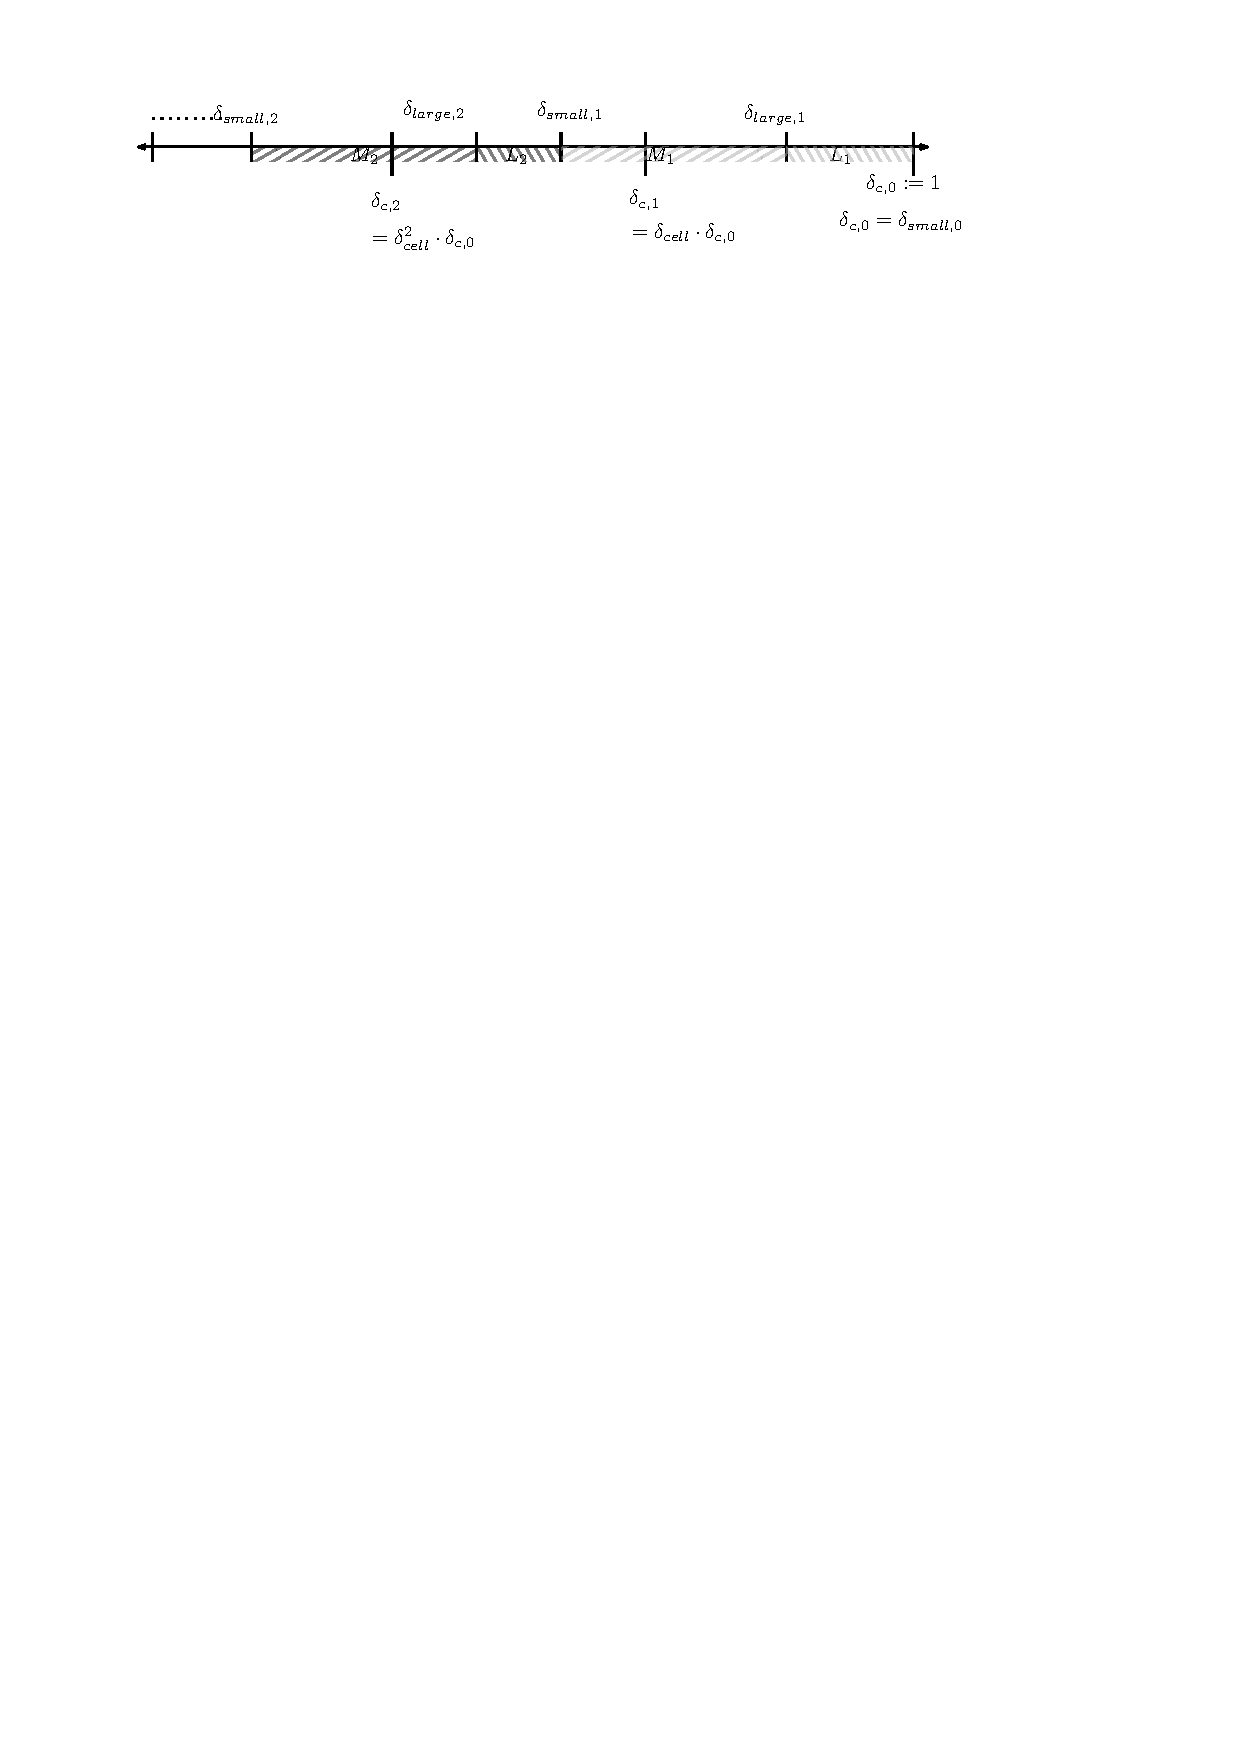
\includegraphics[width=\textwidth]{Figures/large_medium_discretized_delta.pdf}
    \caption{Grouping of objects based on \(\delta_{cell},\delta_{small},\delta_{large}\) and the corresponding Large and Medium sets. The line is not to scale.}
    \label{fig:large-medium-discretized}
\end{figure}

Note that our grid and the sets $L_{\ell}$ and $M_{\ell}$ depend
on the (initial) choice of $\dl, \ds$ and $\dc$. (See Figure~\ref{fig:large-medium-discretized} for an illustration.) In the next lemma, we show via
a shifting argument that there are choices for these values such that the
total area of the objects in $\bigcup_{\ell}M_{\ell}$ is very small.
This will allow us later to pack them separately via a simple greedy
algorithm. In particular, these choices are from a set of $O_\eps(1)$ candidate values $D$, and thus
we will be able to guess them later easily.


\begin{lemma}\label{lem:medium-items}Let $f\ge 1$. There is a global set $D$ with $|D|\le O_{\eps,f}(1)$
such that for any set of $f$-fat convex objects $\P$ that can be packed
in a knapsack $K=[0,1]\times[0,1]$, there are values $\dl,\ds,\dc>0$
that are all contained in $D$
such that for the resulting hierarchical grid and the corresponding
sets $\left\{ L_{\ell},M_{\ell}\right\} _{\ell}$ we have that the
total area of all objects in $\bigcup_{\ell}M_{\ell}$ is bounded
by $\eps$ (and thus corresponding in-radius is less than $\eps$).
\end{lemma}

%\subsection{Proof of \Cref{lem:medium-items}}
\begin{proof}
This follows from a shifting argument similar to Lemma \ref{lem:shifting}. 
Say, we need $\ds \le \dc \le \dl$ such that $\ds \le \beta \dc, \dc \le \gamma \dl$, for some constants $\beta, \gamma \in (0,1]$. 

Define $\rho_0 := 1$, %(\beta \gamma)^{1/\eps} \cdot \eps/f$, 
and $\rhoi{k} := \beta \gamma \cdot \rho_{k-1}$. For each integer $k \in [2/\eps]$ 
\arir{to make sure $\dl, \dc$ is sufficiently small such that medium items have small radius and can fit in the augmented region of $\eps$ width. Another simpler option might be just to show the area of medium to be $\eps^2$ instead of $\eps$, by using more classes.
We can also start with $\rho_0=\eps^2$ but then $\delta_{c,\ell} \neq \dc \delta_{c,\ell-1}$ for all $\ell$.}
we define the following sets of items as shown in \Cref{fig:split}:
\begin{align*}
\mathcal{C}_k = \{C_i \in \mathcal{P} \mid r^{in}(C_i) \in \bigcup_{j=1}^{\infty} (\rho_{k},\rho_{k-1}]\cdot (\beta \gamma)^{(2j/\eps)}\}.
\end{align*}

Then, by averaging argument there is a $k \in \{\frac{1}{\eps}+1, \frac{1}{\eps}+2, \ldots, \frac{2}{\eps}\}$  such that the area of $\mathcal{C}_k$ is at most $\eps$.
Define $\dl:=\rho_{k-1}, \dc:=\gamma \dl, \ds:=\beta \dc=\beta \gamma \dl=\beta \gamma \rho_{k-1}=\rho_k$. 
Define $D:= \{{(\beta \gamma)}^{2/\eps}, {(\beta \gamma)}^{2/\eps -1 }\gamma, {(\beta \gamma)}^{(2/\eps)-1}, \dots,  (\beta \gamma)^{1/\eps+1},  (\beta \gamma)^{1/\eps} \gamma, (\beta \gamma)^{1/\eps})\}$.
Clearly, any chosen $\ds, \dc, \dl$ belong to $D$.
Also, as $k \in \{\frac{1}{\eps}+1, \frac{1}{\eps}+2, \cdots, \frac{2}{\eps}\}$, we have $\dc,\dl \le {(\beta \gamma)}^{1/\eps}$. 

Later we will see that choosing \ag{$\beta=\eps^2/16, \gamma=\eps/(72f)$} suffices for our purpose (see proof of \Cref{lem:fatdiscrete}). 
This also ensures that any object in $\cup_{\ell} M_\ell$ has outradius (and thus inradius)  at most $\eps$. 
\end{proof}
\begin{figure}
	\centering 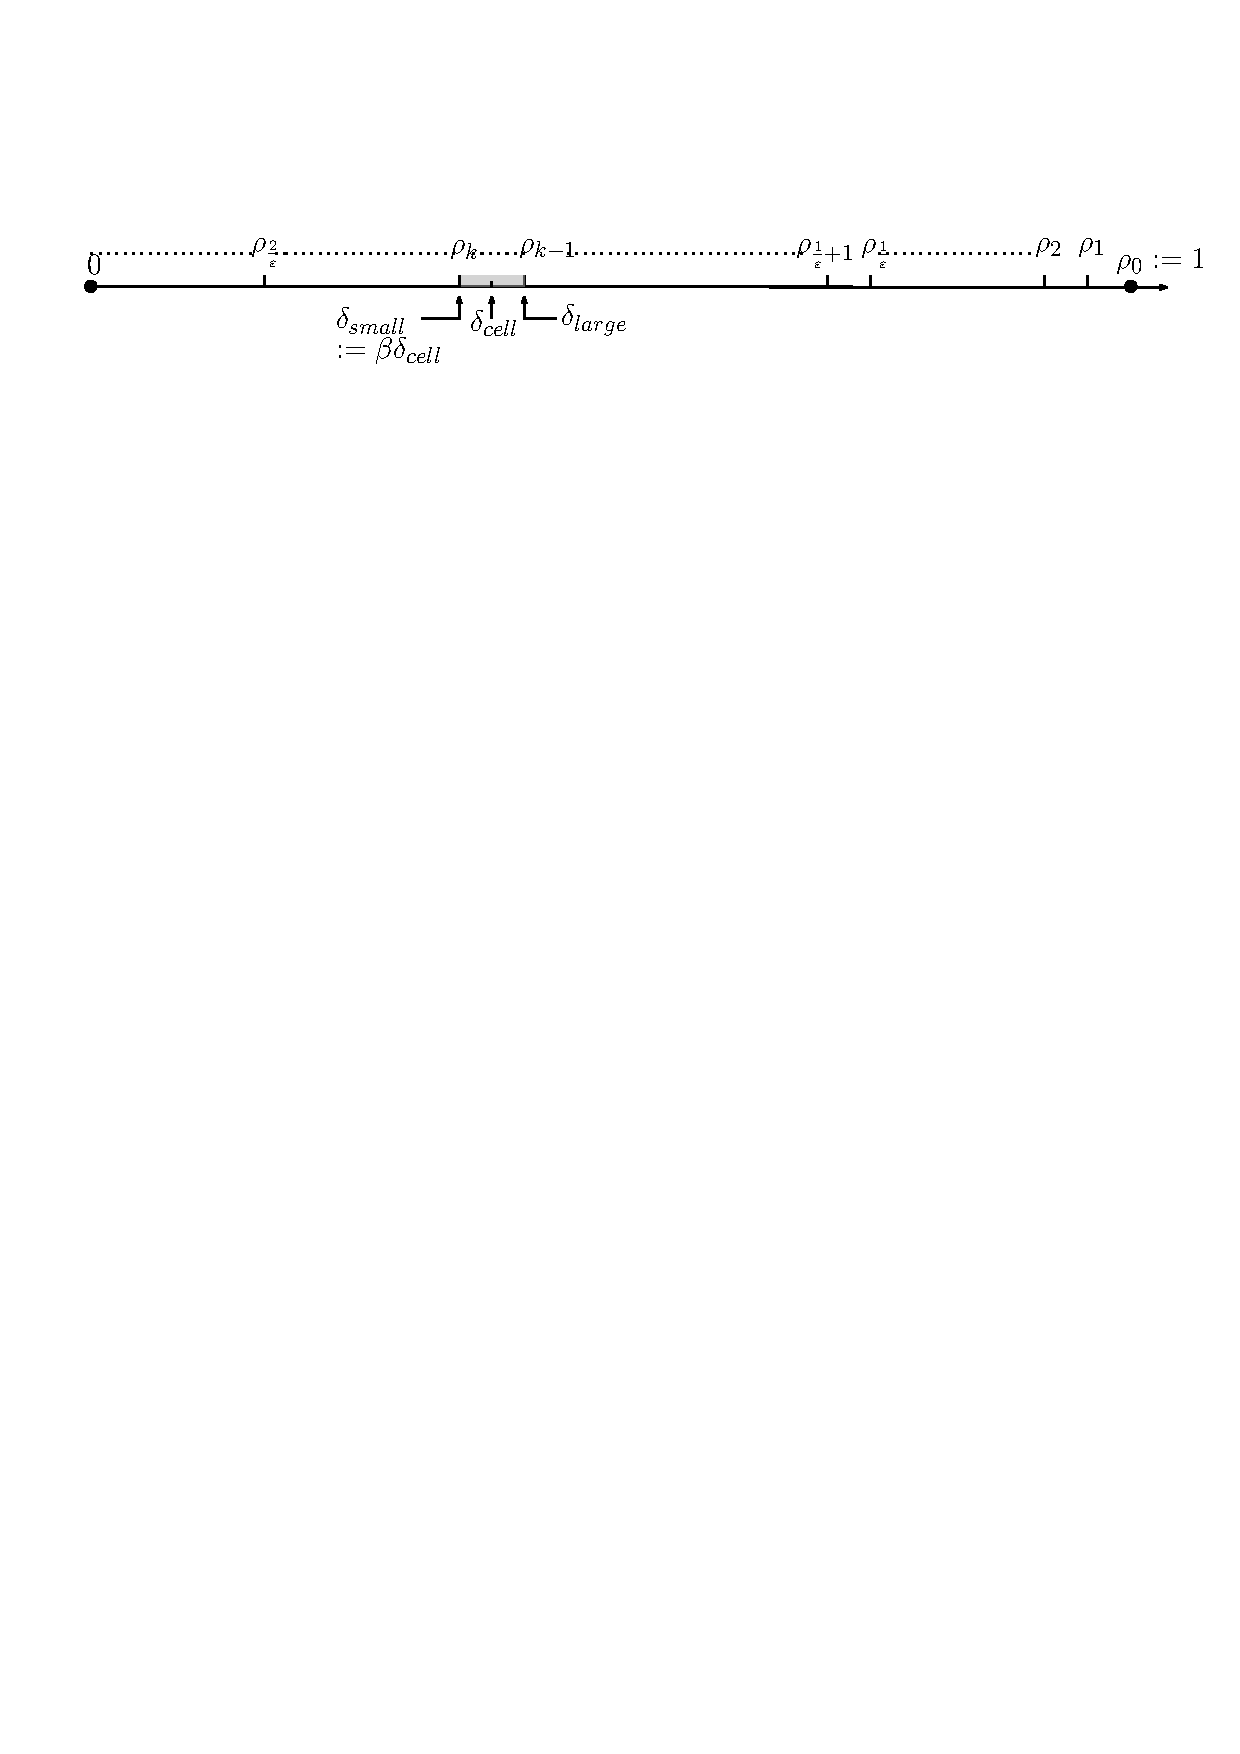
\includegraphics[width=\textwidth]{Figures/aar_figure4}
	% Scale image to the width of the text
	\caption{Splitting of sets $\mathcal{C}_k$ on the real line (not to scale) as used in \Cref{lem:medium-items}.}
	\label{fig:split}
\end{figure}
%%%%%%%%%%%%%%%%

We generalize now our notion of discretized packings. Intuitively,
like before, we require that there is a partition of the grid cells
such that for each object $P\in\P$ there is a set of grid cells $\G_{P}$
that contain $P$ and that are disjoint from the grid cells $\G_{P'}$
for each object $P'\in\P\setminus\{P\}$. Formally, we define that
our packing of $\mathcal{P}$ is \emph{discretized} if
\begin{itemize}
\item for each level $\ell$ and for each object $P\in\mathcal{P}\cap L_{\ell}$
there is a set of $O(1/\dc^{2})$ grid cells
$\mathcal{G}_{P}$
of level $\ell$ such that $P$ is contained in $\mathcal{G}_{P}$,
and there is a single grid cell of level $\ell-1$ that contains all
grid cells in $\mathcal{G}_{P}$, and
\item for any two objects $P,P'\in\mathcal{P}$ (not necessarily of the
same level) and for any two grid cells $C\in\mathcal{G}_{P}$ and
$C'\in\mathcal{G}_{P}'$ their relative interiors are disjoint.
\end{itemize}
We show that by increasing the size of our knapsack by a factor of
$1+\eps$, there is a discretized packing for all objects in {$\bigcup_{\ell}L_{\ell}$}.
% the sets $L_i$.
As mentioned above, we will pack the objects in {$\bigcup_{\ell}M_{\ell}$}
separately later. %


\begin{lemma}%[$\star$] 
	\label{lem:fatdiscrete} Let each $f\ge1$ and $\eps>0$.
There is a global set $D$ with $|D| \le O_{\eps,f}(1)$ such that for
any set of $f$-fat objects $\mathcal{P}$ that can be placed non-overlappingly
inside a knapsack $K=[0,1]\times[0,1]$, there is a choice for the
grid with parameters $\dl,\ds,\dc>0$ such that all these values are
contained in $D$ and there is a discretized packing for $\mathcal{P}\cap (\bigcup_{\ell}L_{\ell})$
inside an (augmented) knapsack \ari{$[0,1+O(\eps)]\times[0,1+O(\eps)]$}. \end{lemma}

\begin{proof}
	We start with the given packing of $\mathcal{P}$ in $K$ and do a
	sequence of refinements which leads to our discretized packing for
	$\mathcal{P}\cap\bigcup_{\ell}L_{\ell}$. First, we use the increased
	size of the knapsack to ensure that for each level $\ell$ and any
	two objects $P,P'\in L_{\ell}$, the distance between $P$ and $P'$
	is at least $2\delta_{c,\ell}$. Intuitively, increasing the size
	of the knapsack by a factor of $1+\eps$ is equivalent to shrinking
	the objects in $\mathcal{P}$ by a factor of $1+\eps$. Therefore,
	we can achieve this required minimum distance of $2\delta_{c,\ell}$
	by choosing $\dc$ \ag{appropriately according to the multiple constraints given in the proof of  \Cref{lem:fatdisc}}.
	
	
	Next, we would like that for each level $\ell$, each object in $\mathcal{P}\cap L_{\ell}$
	is contained in a grid cell of level $\ell-1$. This might not be
	the case, however, via a shifting argument (giving the grid a random
	shift) we can argue that this is the case for almost all objects in
	$\mathcal{P}$.
 Any object in $\mathcal{P}\cap L_{\ell}$ has diameter at most $2f \delta_{small,\ell-1}$. 
	\ag{Hence, the probability that an object in level $\ell$ intersects a grid line from level $\ell-1$ is at most \ari{$8f\delta_{small,\ell-1}/\delta_{cell,\ell-1}= 8f\ds/\dc$}.
		Let this probability be smaller than $\eps^2/2$, leading to a constraint \ari{$\ds \leq \eps^2\dc/16f$} on the choice of $\dc,\ds$. Then the total area of intersecting objects must also be smaller than $\eps^2$ as the area of all packed objects can be at most the area of \agtwo{the} augmented knapsack.
	}
 
	Thus we can easily pack these intersected objects into extra
	space that we gain via increasing the size of the knapsack (i.e.,
	for a second time).
	
	After this preparation, we process the objects $P\in\mathcal{P}$
	level by level and define their corresponding sets $\mathcal{G}_{P}$,
	starting with the highest level. Consider a level $\ell$. For each
	object $P\in\mathcal{P}$ of level $\ell$ we define $\mathcal{G}_{P}$
	to be the set of all grid cells of level $\ell$ that intersect with
	$P$. Due to our minimum distance between any two objects in $\mathcal{P}$
	of level $\ell$, for any two different objects $P,P'\in\mathcal{P}$
	of level $\ell$ we have that $\mathcal{G}_{P}\cap\mathcal{G}_{P'}=\emptyset$.
	Now it could be that a cell $\texttt{C} \in\mathcal{G}_{P}$ for some $P\in\mathcal{P}$
	intersects not only with $P$, but also with another object $P'\in\mathcal{P}$
	of some deeper level $\ell'>\ell$. We call such a cell $\texttt{C}$ \emph{problematic};
	recall that we wanted the cells in $\mathcal{G}_{P}$ to be used exclusively
	by $P$. Therefore, we move all objects $P'\in\mathcal{P}$ of some
	level $\ell'>\ell$ that intersect a problematic grid \agtwo{cell} in $\mathcal{G}_{P}$.
	We pack them into extra space that we gain due to resource augmentation.
	We do this operation for all levels $\ell$.
	
	In the process above, we move objects that intersect the problematic grid
	cells. We need to argue that the total area of these moved objects
	is small compared to the size of the knapsack and that, therefore,
	we can pack them into additional space that we gain due to our resource
	augmentation. In particular, we need to argue this globally, over
	all levels. The key insight is that if we define a set $\mathcal{G}_{P}$
	for some object $P\in\mathcal{P}$ as above, then each problematic
	cell $\texttt{C}  \in\mathcal{G}_{P}$ must intersect the boundary of $P$ and,
	since $P$ is fat, the number of problematic cells $ \texttt{C} \in\mathcal{G}_{P}$
	is very small compared to the number of cells $\texttt{C}' \in\mathcal{G}_{P}$
	that are contained in $P$ and, thus, for sure \emph{not }problematic.
	
	\arir{Check these calculations}
	\ari{By the classical {\em Barbier's theorem}, we know  the perimeter of a convex set $P$ of level $\ell$ is at most $\pi \cdot \text{diameter}(P) \le 2\pi r^{out} \le 2\pi f r^{in}$.}
	\ag{A curve of length $\delta_{cell, \ell}$ is bound to be contained inside a circle of radius $\delta_{cell, \ell}$. This implies that this curve can intersect at most $9$ grid cells as any circle of radius $\delta_{cell, \ell}$ can be bounded in a $3\times 3$ grid cells of side length $\delta_{cell, \ell}$.}
	\ag{
		Hence, the number of grid cells (of level $\ell$) $N_1$ that the perimeter can intersect is at most $18\pi f r^{in}/\delta_{cell,\ell}$. }
	\ari{
		On the other hand, $P$ completely contains at least grid cells of area $\pi (r^{in}-2\delta_{cell, \ell})^2$, 
		i.e., the number of such gridcells $N_2$ is at least $\frac{\pi (r^{in}-2\delta_{cell, \ell})^2}{(\delta_{cell, \ell})^2}$.
		We need $N_1 \le \eps N_2$.}
	\ag{Equivalently, we want to show, $\delta_{cell, \ell} \le \frac{\eps}{18f} \cdot \frac{(r^{in}-2\delta_{cell, \ell})^2}{r^{in}}$.
		For this we impose the condition that $\dl \ge \frac{72f}{\eps} \dc$.
		Then, $\frac{\eps}{18f} \cdot \frac{(r^{in}-2\delta_{cell, \ell})^2}{r^{in}} \ge \frac{\eps}{18f} \cdot \frac{(r^{in}/2)^2}{r^{in}}\ge  \frac{\eps}{18f} \cdot \frac{\delta_{large, \ell}}{4} \ge \delta_{cell, \ell}$.}
	
	
	
	Using this, we derive a \emph{global }argumentation, stating that
	the total area of \emph{all} problematic grid cells over all objects
	of all levels is at most an $\eps$-fraction of the area of the
	knapsack. Also, if an object $P'$ of some level $\ell'$ intersects
	a problematic grid cell $\texttt{C}$ of some level $\ell<\ell'$, then $P'$
	is very small compared to $\texttt{C}$. Thus, the total area of these objects
	intersecting a problematic grid cell $\texttt{C}$ is essentially the same
	as the area of $\texttt{C}$. Thus, we can pack all these objects into our
	additional space due to resource augmentation.
	
	Finally, we can afford to increase the space of our knapsack such
	that this additional space is even by a constant factor larger than
	the total area of the objects we need to pack into it. Therefore,
	it is easy to find a discretized packing for them in this extra space.
\end{proof}


One can easily extend the above lemma to the case of $O(1)$ number of knapsacks.
\begin{corollary}
\label{corr:fatdiscrete} Let $f\ge1$, $\eps>0$, and $c_m$ be constants.
There is a global set $D$ with $|D|$ to be $ O(1)$ (the constant is independent of $n$ and only depends on $\eps, f, c_m$) such that for
any set of $f$-fat objects $\mathcal{P}$ that can be placed non-overlappingly
inside $c_m$ square knapsacks with side length 1, there is a choice for the
grid with parameters $\dl,\ds,\dc>0$ such that all these values are
contained in $D$ and there is a discretized packing for $\mathcal{P}\cap (\bigcup_{\ell}L_{\ell})$
inside $c_m$ (augmented) knapsacks of side length $1+\eps$ each. 
\end{corollary}
%\awr{If we write  $|D| \le O_{\eps}(1)$  then it looks as if $D$ does not depend on $f$ and $c_m$. Is this the case? == changed.}

\noindent \textbf{Algorithm.} \ari{Now we describe our algorithm. First, we {\em correctly} guess (i.e., by brute-force enumeration of all possible cases) the values $\dl,\ds,\dc>0$ from set $D$
 due to Lemma~\ref{lem:fatdiscrete}. 
Note that we still do not know $\bigcup_{\ell} L_{\ell}$ or $\bigcup_{\ell} M_{\ell}$, i.e., which objects are there in the optimal packing. 
So, for each level $\ell$ we define
$\tilde{L}_{\ell}$ to be all input objects
$P$ with $r^{\ag{in}}(P)\in(\delta_{large,\ell},\delta_{small,{(\ell-1)}}]$ and  
$\tilde{M}_{\ell}$ to be all input objects $P$ with $r^{in}(P)\in(\delta_{small,\ell},\delta_{large,\ell}]$.}
\arir{Used $\tilde{L}_{\ell}$ instead of ${L}_{\ell}$. As  ${L}_{\ell}$ refers to items in optimal packing. Please check the whole para.}

Then, we compute an optimal
discretized packing via a dynamic program. Intuitively, our DP computes
an optimal subset of $\bigcup_{\ell}\tilde{L}_{\ell}$ for which there is a discretized
packing. % Note that we can guess $O_{1/\eps}(1)$ we can guess $\dl, \ds, \dc$.
We introduce a DP-cell % Each cell in our DP-For the correct guess, let the DP-cell is
$\DP[\ell,m]$ for each combination of a level $\ell$ and a value
$m\in\{1,...,n\}$. This cell corresponds to the subproblem of packing
a maximum profit subset of the objects in $\tilde{L}_{\ell},\tilde{L}_{\ell+1},\tilde{L}_{\ell+2},\dots.$
via a discretized packing into at most $m$ grid cells of level $\ell-1$,
i.e., with side length $\delta_{c,(\ell-1)}$ each. Recall that each
object in $\tilde{L}_{\ell}$ is relatively large compared to the grid cells
of level $\ell-1$. Therefore, we can pack only constantly many items
from $\tilde{L}_{\ell}$ into each of these $m$ grid cells of level $\ell-1$.
Hence, there are only constantly many options for how the set $\mathcal{G}_{P}$
of an object $P\in \tilde{L}_{\ell}$ in the optimal solution to our subproblem
can look like. We say that a \emph{configuration} is a
partition of a grid cell of level $\ell-1$ into sets of grid cells of level $\ell$.
Each grid cell of level $\ell-1$ contains
{$O(1/\dc^2)$ many grid cells of level $\ell$. Hence, there are only constantly
many configurations.
% such that the union
% of the grid cells in $\mathcal{G}'$ is contained in a grid cells
% of level $\ell-1$.
We assume two configurations to be \emph{equivalent} if they are identical up to translation by an integral multiple of $\delta_{c,(\ell-1)}$, i.e., by an integral multiple of the edge length of a grid cell of level $\ell-1$.
%  Thus, for our $m$ grid cells of level $\ell-1$ there
% are only constantly many configurations, at most \ari{$2^{O(1/\dc^2)}$} many.
Denote by $C$ the total number of resulting equivalence classes.
We guess in time $m^{O(C)}\le n^{O(C)}$ how many grid cells
have each of the at most $C$ configurations (up to equivalences). Then, we assign the
items in $\tilde{L}_{\ell}$ into the grid cells according to this guess.
\ari{We can do this by weighted bipartite matching. For each object
$P\in \tilde{L}_{\ell}$, each possible configuration $\mathcal{G}'$, and each set in the partition of
$\mathcal{G}'$, we
can check easily whether $P$ fits into $\mathcal{G}'$. 
In the bipartite graph, one side will contain the objects in $\tilde{L}_{\ell}$ and the other side will contain the sets in the partition of
$\mathcal{G}'$.
If $P$ fits into set $Q$ in the \agtwo{partition} of $\mathcal{G}'$, then there is an edge with edge cost as $\profit(P)$. }
Our guess
yields a certain number $m'$ of empty grid cells of level $\ell+1$
into which we need to pack items in $\tilde{L}_{\ell+1},\tilde{L}_{\ell+2},\dots$.
We assign these items according to the solution in the DP-cell $\DP[\ell+1,\min\{m',n\}]$.
Note that there are at most $n$ items and, hence, we never need more
than $n$ grid cells of level $\ell+1$. Also, since our input data is
polynomially bounded, the number of classes $\tilde{L}_{i}$ is bounded
by~$n^{O(1)}$. Thus, our DP runs in time $n^{O(C)}$.

Additionally, we pack medium objects from the set $\bigcup_{\ell}\tilde{M}_{\ell}$
separately in a strip of the form $[0,1]\times[1,1+O(\eps)]$. We select the most profitable subset of $\bigcup_{\ell}\tilde{M}_{\ell}$
(up to a factor of $1+\eps$) whose total area is bounded by $\eps$
(see Lemma~\ref{lem:medium-items}).
% ,
% i.e., the area of the strip $[0,1]\times[1,1+\eps]$.
We replace each
of these objects with the smallest square that contains it, which
increases its area only by a constant factor.
We can pack these squares efficiently into a (slightly larger) strip $[0,1]\times[1,1+O(\eps)]$ using the $\mathtt{NFDH}$ algorithm~\cite{NFDH}. This yields the following lemma.
% Now we state a result that gives an approximation algorithm for packing small squares of total area $O(\eps$) efficiently.

% \begin{lemma}[\cite{NFDH}]\label{lem:nfdh}
% 	In a rectangle of size $a \times b$, the $\mathtt{NFDH}$ algorithm guarantees to pack an area of at least $(ab-\mu(a+b))$ with sufficient number of squares of maximum side length $\mu$.
% \end{lemma}
%
%%\cite{NFDH} stated in \Cref{lem:nfdh} into a (slightly larger) strip $[0,1]\times[1,1+O_f(\eps)]$ to arrive at the following lemma.

\begin{lemma}
\label{lem:med}
In polynomial time we can compute a set $\P'\subseteq \bigcup_{\ell}\tilde{M}_{\ell}$
and a non-overlapping placement of $\P'$ inside $[0,1]\times[1,1+O(\eps)]$
such that $w(\P')$ is at least the profit of any subset of \ari{$\bigcup_{\ell}\tilde{M}_{\ell}$}
whose total area is at most $\eps$.
\end{lemma}

\begin{proof}
Let the most profitable subset of $\bigcup_{\ell} \tilde{M}_{\ell}$
(up to a factor of $1+\eps$) whose total area is bounded by $\eps$ be $\OPT_{M}$.
 We arrange all items in $\bigcup_{\ell}\tilde{M}_{\ell}$ in order of decreasing profit density and select (prefix) subset of items with highest profit density such that their area is bounded by $2\eps$. Let this subset of items be $M'$. We argue that $w(M')\ge w(\OPT_M)$ as any items in $\bigcup_{\ell} \tilde{M}_{\ell}$ has area at most $\eps$.
 Therefore, our selected set $M'$ has profit at least $\profit(\bigcup_{\ell}M_{\ell})$
(see Lemma~\ref{lem:medium-items}).
Now we pack  $M'$ 
separately in a strip of the form $[0,1]\times[1,1+O(\eps)]$.
% ,
% i.e., the area of the strip $[0,1]\times[1,1+\eps]$.
We replace each
of these objects with the smallest square that contains it, which
increases its area only by a constant factor of at most {$2f^2$ since each item is $f$-fat. Note that this square has a side length of at most $2r^{out} \le 2f r^{in} \le 2f\eps$ as all the medium objects have an inradius of at most $\eps$. Now we state a result that gives an approximation algorithm for packing small squares of size $O(\eps$) efficiently.}
\begin{lemma}[\cite{NFDH}]\label{lem:nfdh}
	In a rectangle of size $a \times b$, the $\mathtt{NFDH}$ algorithm guarantees to pack an area of at least $(ab-\mu(a+b))$ with a sufficient number of squares of maximum side length $\mu$.
\end{lemma}

We pack these square objects greedily with the $\mathtt{NFDH}$ algorithm
\cite{NFDH} stated in \Cref{lem:nfdh} into a (slightly larger) strip $[0,1]\times[1,1+O_f(\eps)]$ to arrive at the result we wanted to prove.
\end{proof}
%%%%%%%%%%%%%%%
%\awr{added the following theorem to handle multiple knapsacks}
The algorithm is easy to extend to the case of a constant number (say, $c_m$) of knapsacks. For a single knapsack, we call DP[0,1], whereas for multiple knapsacks we need to just call DP[0,$c_m$]. This leads to the following corollary. 

\begin{corollary}
	\label{cor:fat-ra}
	Let \ari{$f\ge 1$}, $\eps>0$, $d\in \N$, and $c_m$ be constants. Given a set of $d$-dimensional $f$-fat convex input objects, there exists a polynomial time algorithm that can pack a subset of them with a total profit of \ag{$w(\OPT)$} into $c_m$ knapsacks with side length $1+\eps$, where \ag{$w(\OPT)$} is the optimal profit that can be packed into $c_m$ knapsacks with side length 1.
\end{corollary}
%%%%%%%%%%%%
%%%%%%%%%%%

One can easily extend our algorithm above to any constant dimension $d$.
This completes the proof of \Cref{thm:fat-ra}. %\Cref{thm:fat-ra}.


A consequence is that we obtain a polynomial time $(1+\eps)$-approximation
\emph{without }resource augmentation if all input objects are small,
i.e., if $r^{out}(P)\le\eps$ for each given object $P\in\P$.
Using this property, we can argue that there is a $(1+\eps)$-approximate solution
in which only the area $[0, 1-\Theta(\eps)]\times[0, 1-\Theta(\eps)]$ of the
knapsack is used. Thus, we can use the free space for the resource augmentation
that is required by our algorithm due to \Cref{thm:fat-ra}.


\begin{theorem}
\label{lem:small-poly}
Let $d\in \N$ be a constant.
There is a polynomial time $(1+O(\eps))$-approximation
for the geometric knapsack problem if the set of input objects $\P$
consists of convex fat $d$-dimensional objects such that $r^{out}(P)\le\eps$
for each $P\in\P$.
\end{theorem}

\begin{proof}
We begin by assuming that the optimal solution for this problem is $\OPT$. We then remove two randomized strips of width $\eps$.
First, we select an $x,y \in [0,1-\eps]$ uniformly at random. Then we remove all items that intersect the horizontal strip $[0,1]\times [x, \eps]$ and all items that intersect the vertical strip $[x, \eps] \times [0,1]$. 
Each item is then cut with probability at most $2(2 r^{out}+\eps)$. 
In expectation, then we incur a loss of at most $2(2 r^{out}+\eps) \le 6 \eps$ fraction of the profit. 
This can also be derandomized by an averaging argument. 
From this, we get a packing of $(1-O(\eps)) \ag{w(\OPT)}$ profit in a $(1-\eps)\times (1-\eps)$ bin. We now use Theorem~\ref{thm:fat-ra} to get this packing from the set $\P$ in polynomial time. 
\end{proof}